\documentclass[12pt,paperletter]{article}
\usepackage[activeacute,spanish,es-noquoting]{babel}
\usepackage[letterpaper,includeheadfoot, top=1.5cm, bottom=1.5cm, right=2.0cm, left=2.0cm]{geometry}
\usepackage{wrapfig}
\usepackage{amsmath}
\usepackage{amsthm}
\usepackage{bbold}
\usepackage{color}
\usepackage{xcolor}
\usepackage{graphicx}
\usepackage{float}
\usepackage{amssymb}
\usepackage{dsfont}
\usepackage{parcolumns}
%\usepackage{pdfpages}
\usepackage{fancyhdr}
\usepackage{float}
\usepackage{subfig}
\usepackage{hyperref}
\usepackage{pgf,tikz}
\usetikzlibrary{arrows}
%Pseudocodigo
\usepackage{algpseudocode}
\usepackage{algorithm}
\usepackage{pseudocode}
\usepackage{varwidth}
\usepackage{dsfont}
\usepackage{enumerate}
\usepackage{tikz}
\usepackage{listings} %escribir código.
\usepackage{diagbox} %tablas doble entrada
\usepackage[utf8]{inputenc}
\usepackage{comment}
\usetikzlibrary{automata,positioning}
\usepackage{pgfplots}
\pgfplotsset{compat=newest}
%Regla
\newcommand{\horrule}[1]{\rule{\linewidth}{#1}} % Create horizontal rule command with 1 argument of height

\newcommand{\NaN}{\texttt{NaN}}
%=====================================
%\usepackage[framed,numbered,autolinebreaks,useliterate]{mcode}
\graphicspath{{images/}{otherfolder/}}

%INDENTACION
%\setlength{\parindent}{0pt}
%============INFORMACION==================
\newcommand{\profeA}{Axel Osses}
\newcommand{\profAuxA}{Pablo Arratia}
\newcommand{\profAuxB}{Manuel Suil Jorquera}
\newcommand{\alumnoA}{Guillermo Dinamarca}
\newcommand{\alumnoB}{Edgar Contreras Mayr}
\newcommand{\dpto}{Departamento de Ingeniería Matemática}
\newcommand{\curso}{MA5307-1 Análisis Numérico de Ecuaciones en Derivadas Parciales: Teoría y Laboratorio}
\newcommand{\TareaNum}{}
\newcommand{\tituloLab}{Propagación de calor en un medio heterogéneo: aplicación a fuentes de calor domésticas}
\newcommand{\fecha}{\today}
%=====================================
\newcommand{\R}{\mathbb{R}}

\renewcommand{\baselinestretch}{1.3}

%Redefinición Demostración
\renewcommand{\qedsymbol}{\rule{0.7em}{0.7em}}
%\usepackage[biblabel]{cite}
\renewenvironment{proof}{{\bfseries \noindent Demostración}}{ \qed \\}
%==========================================
\newcommand{\s}{\sigma}
\renewcommand{\t}{\tau}
\newcommand{\Om}{\Omega}
\newcommand{\h}{\mathbf{H}}
\newcommand{\om}{\omega}
\newcommand{\tgt}[1]{\texttt{#1}}
\newcommand{\N}{\mathds{N}}
\newcommand{\imp}{\Rightarrow}
\newcommand{\RR}{\mathds{R}}
\newcommand{\noi}{\noindent}
\renewcommand{\O}{\Omega}
\newcommand{\ds}{\displaystyle}
\usepackage{cancel}
\renewcommand{\thesubsection}{\thesection.\arabic{subsection}}
\renewcommand{\thesubsubsection}{Ejercicio \arabic{subsubsection}}
%Para comenzar las subsubsecciones desde un número arbitrario
\newcommand{\subsubnum}[1]{\setcounter{subsubsection}{#1 - 1}}
\begin{document}
\setlength{\parindent}{0pt}
%\input{commands}
\newtheorem{exercice}{\bf Ejercicio}
\newenvironment{ejercicio}{\begin{exercice}
\rm}{\end{exercice}}
\def\matlab{{\tt Matlab\ }}
\def\python{{\tt Python\ }}
%\input{header}



%\begin{sf}
%==============PORTADA=====================
%Paquete para dibujos en latex
\usepackage{tikz}


%\begin{titlepage}
\pagestyle{fancy}
\fancyhf{}

%==============CABECERA=====================
\renewcommand{\headrulewidth}{1pt}
\fancyhead[L]{\begin{wrapfigure}{l}{0.2\textwidth}
  \begin{center}
  \advance\leftskip 0cm
  \vspace{-1.5cm}
    
\includegraphics[width=0.2\textwidth]{fcfm.pdf}
  \end{center}
\end{wrapfigure}
\large \textbf{Universidad de Chile} \\ \text{Facultad de Ciencias Físicas y Matemáticas} \\ \text{\dpto} \\ \text{MA5307-1 Análisis Numérico de Ecuaciones en Derivadas Parciales}}


%==============TITULO=====================

\vspace*{7cm}
\begin{center}
%\horrule{1pt} \\[0.5cm] % Thin top horizontal rule
\Huge Informe de Proyecto:  \\[0.2 cm] % The assignment title
\LARGE  \tituloLab \\
%\horrule{1pt} \\[0.5cm] % Thick bottom horizontal rule
\vspace{0.2cm}
\huge{}
\end{center}

%===============NOMBRES====================
\vfill
\begin{flushright}
\begin{tabular}{lll}
Nombres:  & \alumnoA \\
          & \alumnoB  \\ \\
Profesor de Cátedra: 	& \profeA \\ \\
                        %& \profeB \\ \\
Profesor Ayudante: 	& \profAuxA \\
                    & \profAuxB \\
%Profesor Ayudante:	& \ayudante \\ 
%                   & \ayudanteB \\ \\
Fecha: & \fecha \\
\end{tabular}
\end{flushright}
%\end{titlepage}
\newgeometry{top=2.5cm, bottom=2.5cm, right=2.0cm, left=2.0cm}
\newpage
\pagestyle{fancy}
\fancyhf{}
%Encabezado
%\fancyhead[L]{\rightmark}
\fancyhead[L]{\small \rm \textit{\curso}} %Izquierda
\fancyhead[R]{\small \rm \textit{}} %Derecha
%\fancyfoot[L]{\small \rm \textit{Tarea \TareaNum}} %Izquierda
\fancyfoot[R]{\small \rm \textbf{\thepage}} %Derecha
%\fancyfoot[C]{\thepage} %Centro
\renewcommand{\sectionmark}[1]{\markright{\thesection.\ #1}}
\renewcommand{\headrulewidth}{0.5pt}
%\renewcommand{\footrulewidth}{0.5pt}

\tableofcontents

\newpage
\section{Introducción}

En este proyecto se aborda el problema de propagación de calor, este proceso se conoce como difusión de calor, se estudia el proceso de como se calienta una una casa mediante la acción de una o más estufas en posiciones arbitrarias. Para simplificar el problema, la casa es de un piso, y consta de paredes rectas y ángulos rectangulares en las esquinas, además se considera una vista aérea de la casa. \\

Para comenzar el estudio se comienza planteando una ecuación que modele el fenómeno físico que se quiere estudiar, para ello se usa el proceso de difusión del calor y se consideran las funciones que aportan calor al sistema, en este caso son las estufas que se consideran como un punto en el interior del dominio (dominio rectangular).\\

Inicialmente para la parte práctica, se estudia el caso de una habitación y una estufa con alguna apertura o puerta en alguna pared; posteriormente se desarrolla un programa capaz de soportar una geometría arbitraria en 2D.\\

La difusión de calor se modela mediante la ecuación del calor, por lo que se realiza la formulación variacional del problema para que luego se pueda aplicar el método de Elementos Finitos para resolver de forma numérica el problema.

\newpage
\section{Marco teórico}

\subsection{Modelación del problema}
Se considera la ecuación del calor como base para la resolución del problema. La idea es establecer condiciones de borde que representen adecuadamente las paredes de la casa y agregar fuentes de calor en la ecuación que modelen la emisión de calor dada por la estufa. 

Sea $q_t(R)$ la tasa de flujo de calor hacia una región $\O$. Si $q$ tiene densidad $Q$, tenemos que $$q_t(R) = \int_\O Q(x,t)$$

El flujo de calor es una función vectorial $\mathbf{H}(x)$, que caracteriza a $q_t$ como sigue: la tasa $q_t$ fluyendo por un elemento infinitesimal de área $dS$ y vector normal $n$ es $\h(x) \dot n(x) dS$. Así, tenemos que 
$$q_t(R) = -\int_R \h(x)n(x)dS$$

Según la ley de Fourier, el flujo de energía depende linealmente del gradiente de la temperatura:

$$\h(x) - A(x)\cdot \nabla u(x)$$

donde $A(x) \in \R^{3\times3}$ es simétrica y definida positiva, y depende de la conductividad términa del medio en las distintas direcciones.\\

Además, sabemos que el cambio de temperatura en $x$ es proporcional al calor fluyendo hacia $x$

$$\partial_t u(x,t) = \kappa(x) Q(x,t)$$

donde $\kappa(x) = \dfrac{1}{\rho(x) C_p(x)}$, con $\rho$ la densidad y $C_p$ el calor específico del medio en $x$.

Consideramos también fuentes de calor puntuales $f(x) = \sum_{j} T_j\delta_j(x)$, donde $T_j$ es la temperatura de la fuente $j$ y $\delta_j = \mathds{1}_{x = x_j}$ es la delta de Kronecker en $x_j$ la posición de la fuente.

Combinando las ecuaciones anteriores tenemos la ecuación general de flujo de calor:

\begin{align}
    \label{eqn:gnral}
     \partial_t u(x,t) - \kappa(x) \sum_{i,j}\partial_{x_i}(a_{ij}(x)\partial_{x_j} u(x,t)) = f(x)
\end{align}

En este proyecto asumimos que cada pared es homogénea isotrópica, por lo que el medio es homogéneo isotrópico por pedazos. Esto implica que $A(x)$ es una matriz simétrica, diagonal, definida positiva, y constante por pedazos en $x$: por ende, la derivada es $0$ c.t.p. y podemos escribir la ecuación como

\begin{align}
    \label{eqn:2}
    \partial_t u(x,t) - \kappa(x)a(x) \Delta u(x,t) = f(x)
\end{align}

Consideramos además condiciones de borde mixtas $u = T_0 \in \R$ en $\partial \O_D$ (donde $\partial \O_D$ representa las aberturas de la casa) y $\nabla u \cdot \ n = 0$ en $\partial \O_N$. Los resultados teóricos también son válidos para el caso de condiciones de borde de tipo Robin.

Para ver la forma variacional del problema, multimplicamos la ecuación \ref{eqn:2} por una función test $v$: integrando por partes, obtenemos

$$\frac{d}{dt}\int_\O u\cdot v dx + \int_\O \kappa(x) a(x) \nabla u\cdot \nabla v dx + \int_{\partial \O_N} \cancelto{0}{\nabla u\cdot n\  v} = \int_\O f\cdot v$$

\newpage
\section{Resolución numérica}
\subsection{Caso simplificado: Habitación cuadrada}

Se dispuso una habitación cuadrada $\O = [0,1]^2$ con una estufa en la posición $(\frac{2}{7}, \frac{5}{7})$. La habitación tiene una abertura en las coordenadas $y \in [1/3,2/3]$. Las figuras \ref{pieza1} y \ref{pieza2} muestran un instante de la resolución numérica de esta habitación. Los parámetros utilizados (conductividades térmicas, densidades, etc.) corresponden a aire a nivel del mar y paredes de madera.

\begin{figure}[H]
    \centering
    \begin{minipage}{0.45\textwidth}
        \centering
        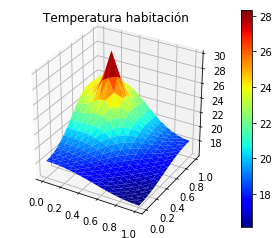
\includegraphics[width=0.9\textwidth]{ejemplo1.png} % first figure itself
        \caption{Instante de la resolución visto en 3D}
    \end{minipage}\hfill
    \begin{minipage}{0.45\textwidth}
        \centering
        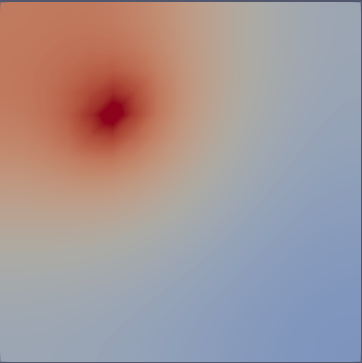
\includegraphics[width=0.9\textwidth]{ejemplo2.PNG} % second figure itself
        \caption{Instante visto desde arriba}
    \end{minipage}
\end{figure}

Se observa que efectivamente el calor fluye desde la fuente hacia los costados, y que los costados cerca de la abertura tienen una temperatura menor.

\subsection{Simulación en una casa arbitraria}

Para extender a un plano general de una casa, se implementan distintas clases en \textit{python}: el dominio y el mallado de éste se general automáticamente a partir de los bloques de aire y las paredes ingresadas, con el cuidado de que las propiedades físicas de las paredes sobreescriban a las de los bloques de aire cuando ocupan el mismo lugar.\\

Como ejemplo, se puede considerar una casa como la siguiente:

\begin{figure}[H]
\begin{center}
    \begin{tikzpicture}
    \draw (0,0.5) -- (2.3,0.5);
    \draw[red,dashed] (1.8,0.5) --(2.8,0.5);
    \draw (2.8,0.5) -- (3.7,0.5)-- (3.7,-1) -- (5,-1) --(5,4) --(0,4) -- (0,0.5);
    \draw[red,dashed] (3.5,4) --(4.5,4);
    \draw (5,2.5) -- (3.7,2.5);
    \draw[red,thick,dashed] (1,2) circle (0.1cm); 
    \draw[red,thick,dashed] (4,-0.5) circle (0.1cm); 
    \end{tikzpicture}
\end{center}
    \caption{Esquema de casa generalizada: dos estufas, dos puertas}
    \label{mapita}
\end{figure}

todas las paredes tienen 0.3 de ancho. Se considera que la geometría de esta casa es lo suficientemente compleja como para comprobar la versatilidad del modelo, y lo suficientemente simple como para entender bien lo que suceda. Ambas estufas están encendidas a la misma temperatura. Se comprueban en la resolución numérica, entre otras cosas, los siguientes puntos:

\begin{itemize}
    \item La pared interior ejerce un efecto aislante que impide el paso de calor a la zona superior derecha
    \item Las entradas abiertas enfrían las zonas cercanas de la casa.
    \item La estufa de abajo a la derecha calienta su entorno más rápido que la de la izquierda, dado que hay menos distancia entre las paredes más cercanas.
\end{itemize}

\begin{figure}[H]
    \centering
    \begin{minipage}{0.45\textwidth}
        \centering
        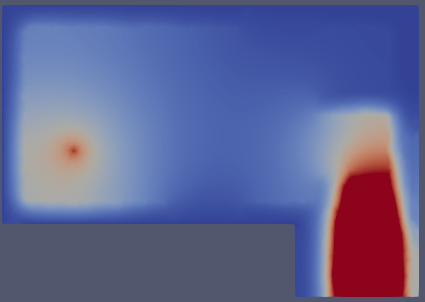
\includegraphics[width=0.9\textwidth]{casa1.PNG} % first figure itself
        \caption{Calor distribuido en la casa, $t\approx \frac{T}{3}$}
    \end{minipage}\hfill
    \begin{minipage}{0.45\textwidth}
        \centering
        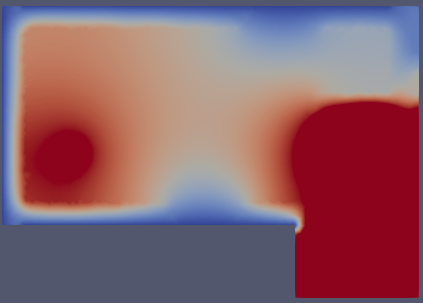
\includegraphics[width=0.9\textwidth]{casa2.PNG} % second figure itself
        \caption{Calor distribuido en la casa, $t\approx \frac{2T}{3}$}
    \end{minipage}
\end{figure}

La resolución numérica (salvo un factor de escala debido seguramente a inexactitud en los parámetros) corresponde con la intuición del problema.



\newpage

\section{Conclusión}




Una vez modelado el problema físico, se reformuló el problema en su forma variacional, lo cual fue de gran ayuda a la hora implementar el modelo en Python. Con esto se pudo ver la potencia y el alcance que tiene el uso de la teoría en conjunto con la parte numérica.\\

El problema de implementación se aborda de forma progresiva, estudiando primero modelos simples, comprendiendo bien las construcciones y las estructuras que se desean programar. Esta metodología lleva a la definición de una clase que sea capaz de crear objetos que representen los componentes de una casa, vale decir: paredes, aire, puertas, estufas. El hecho de poder comprender bien como es que se implementa el programa bien para una habitación simple, permite comprender bien los objetos que van a integrar la clase que se crea, esto hace que el código implementado sea moldeable y fácil de adaptar para crear estructuras más complejas (por ejemplo incorporando paredes de distintos materiales, ventanas, etc.)\\

El proyecto fue una instancia de aprendizaje positiva y su desarrollo contribuyó significativamente en el aprendizaje de las materias del curso.
\end{document}
